\chapter{Related work}
%\section{Dimensionality reduction}
% LLE MDS
\section{Metric learning}
\label{sec:metric_learning}
%Distance metric learning has been a hot topic for a long time in machine learning.
There is a wide range of practical tasks where the estimation of distances or similarities between data points is the central problem. These, for example, include face recognition, person re-identification, document ranking, and also improving the effectiveness of metric-dependent methods, \eg{} k-nearest neighbors and k-means clustering.

Generally, the main goal of building a distance learning framework is to be able to assess the proximity of pairs of objects (here, images) given their feature representations. In more detail, the metric learning method should be able to perform the linear or non-linear mapping of an input space into a new space where the distance between the similar objects should be small, and the distance between the non-similar objects should be substantial. The particular semantics of similarity relation depends on a particular task. 

%todo metntion the intuition of the true mahalanobis metric
\citep{BelletHS13} name three main classes of metric learning tasks in accordance with the available level of  supervision: 
\begin{itemize}
    \item supervised, where the class labels are given for each object, so the objects are considered similar if they belong to the same class \citep{globerson2006metric, NIPS2005_2795, weinberger2009distance},
    \item weakly-supervised, where the similarity labels are given for the pairs of objects \citep{hirzer2012person,koestinger2012large,liao2015person}; it should also be mentioned that for some tasks, the information is given in the form of triplet rankings \citep{schultz2004learning}, 
    \item semi-supervised, where the labels or side information is given for a small number of examples \citep{xing2003distance,davis2007information,mignon2012pcca}.
\end{itemize}
The supervised setting can be considered as having the full side information because in this case, we can generate pairwise labels for every pair in the training set. Additionally, some related works also include more specific scenarios, for example, the case where each object may have several labels, and as a consequence, a pair of objects may have both similar and non-similar labels \citep{GoukPC16}. Generally, the supervision level is defined by the particular problem, \eg{} clustering with the side information implies only knowing which pairs of points should be assigned to the same cluster, for k-NN classification, the full supervision should be available.  % (how is the supervision information related to the following taxonomy???)

In terms of the classification mentioned above, training protocols for face recognition and person re-identification tasks typically imply either supervised setting (\ie{} class labels that correspond to the identities are given) or semi-supervised (\ie{} pairwise labels are given for matching and non-matching pairs of images). The available supervision is most often used to generate the training examples (constraints) of one of the following types: 
\begin{itemize}
    \item pairs \citep{davis2007information,mignon2012pcca,hirzer2012person,koestinger2012large,liao2015person}), \item triplets (\citep{Zheng13}, 
    \item or even quadruplets \citep{law2013quadruplet}. 
\end{itemize}
The methods for metric learning that use more complex types of constraints are not only applicable to classification or verification tasks but may also be used for broader applications that require much richer annotations and therefore cannot be approached using only pairwise constraints. For example, tripletwise constraints allow for ranking problems formulations, whereas quadruplet-based methods can be applied to either ranking problems or hierarchical metric learning. The latter aims at learning  such metric that images from 
sibling classes with respect to the class semantic hierarchy
are more similar than images from more distant classes (\citep{law2013quadruplet}). 
In other words, more flexible types of constraints allow for learning more complex data relations.


%The taxonomy of metric learning methods (\citep{LiT18}) includes several important categories depending on the optimization task formulation: whether the point-wise constraints are used (pairwise, tripletwise), whether the formulation is probabilistic, whether the learned metric is linear or non-linear. The examples of these categories are considered further.


%, whether the solution of the formulated problem is global optimal or local optimal and whether the dimensionality reduction is performed by the method.
%The important features of the metric learning algorithms also include (\citep{BelletHS13}) the scalability with respect to the data dimensionality and to the size of a  training set (number of constraints). Indeed, \citep{weinberger2009distance} and \citep{koestinger2012large} have to apply PCA to reduce the  number of features (up to several hundred) and make the computation feasible, \citep{davis2007information} use feature selection techniques for a similar purpose. %(paisitkriangkrai2015learning --learning to rank)
%\citep{liao2015person} suggests using the specially designed feature descriptor of moderate size. Finally, \citep{mignon2012pcca} state an  optimization problem that allows for learning fewer parameters (linear in the number of input dimensions) which alleviates the problem of using the high-dimensional features. \citep{Qian15} suggests a multistage learning scheme, so that only a part of constraints are to be handled at the same time. 



One important class of distance metric learning algorithms use Mahalanobis distance as it is a generalization of the Euclidean distance that allows for linear feature transformation. Such methods aim at solving an optimization problem with respect to the corresponding positive-semidefinite matrix $\bold{M}$. The goal of such optimization is to pull the similarly labeled points closer and to push further from each other those points that are labeled differently. One of the difficulties of such methods lies in imposing the semi-positive definite matrix for the Mahalanobis distance. To handle this problem, some works suggest iterative schemes including a projection step where the current solution is projected onto the positive semi-definite cone \citep{globerson2006metric,xing2003distance, NIPS2005_2795} or more efficient eigenvalue optimization techniques \citep{ying2012distance}. Some other methods reformulate the task that allows for more efficient solving:  \citep{schultz2004learning} constraint the matrix to be diagonal and thus solve the quadratic program instead of semi-definite one. \citep{hirzer2012person} formulate an optimization problem with equality constraints which allows for closed-form solution.%,  \citep{davis2007information} introduces special regularization term and show that the new formulation is equivalent to low-rank kernel learning.
%\citep{liao2015person} and \citep{hirzer2012person} use the decomposition \ref{eq:mahalanobis_l} that implies positive-semidefiniteness without the need for additional constraints. %, the dimensionality reduction can be easily incorporated by constraining the matrix $L$ to be rectangular. %However, such decomposition makes the optimization problem non-convex; for convex problems, the dimensionality reduction task requires additional low-rank constraints that can make it hard for solving efficiently. 

Non-linear transforms of the initial feature-space can be achieved by kernelization, and some of the Mahalanobis distance learning works \citep{davis2007information,globerson2006metric,NIPS2005_2795,schultz2004learning} suggest the kernelized versions along with the linear ones. 



\bigskip\ident\textbf{Mahalanobis distance learning}\\
\label{sec:mahalanobis}
For the two data points $x_i$ and $x_j$, the Mahalanobis distance is defined as 

\begin{equation}
\label{eq:mahalanobis}
    D_M(x_i, x_j) = \sqrt{(x_i - x_j)\tran \bold{M} (x_i - x_j)},
\end{equation}
where $x_i, x_j \in R^d$, $\bold{M} \in R^{d\times d}$ is a symmetric positive-semidefinite matrix, which ensures that $D_M$ satisfies the pseudo-distance properties. Originally \citep{chandra1936generalised} the term referred to a case when the $\bold{M}$ matrix was equal to the inverse of the sample covariance matrix: $\bold{M} = \sum^{-1}$, but later in metric learning literature, it acquired the broader meaning. 
The goal of the Mahalanobis metric learning methods is to learn the matrix $\bold{M}$. 
Additionally, Mahalanobis distance defined by symmetric positive-semidefinite matrix $\bold{M} = \bold{L}\tran \bold{L}$ can be considered as Euclidean distance after the linear projection $\bold{L}$ of the original inputs:
% \begin{equation}
%  \label{eq:mahalanobis}
% \begin{aligned}

%     D_M(x_i, x_j) = & \sqrt{(x_i - x_j)^T L^T L (x_i - x_j)} = \\ & \sqrt{(L(x_i - x_j))^T L (x_i - x_j)},

% \end{aligned}
% \end{equation}, 

\begin{equation}
  \begin{aligned}
  \label{eq:mahalanobis_l}
    D_M(x_i, x_j) & = \sqrt{(x_i - x_j)\tran \bold{L}\tran \bold{L} (x_i - x_j)} & \\
      & = \sqrt{(\bold{L}(x_i - x_j))\tran \bold{L} (x_i - x_j)} & \\
  \end{aligned}
\end{equation}

which corresponds to simple Euclidean distance in the case of identity matrix $\bold{L}$.


\citep{xing2003distance} are known to suggest the pioneering approach in the metric learning field. The authors aimed at learning Mahalanobis distance to improve the results of clustering with side information. The supervision was given in the form of pairwise constraints defining which data points should be assigned to the same cluster and which of them should be assigned to different clusters. \citep{xing2003distance} formulate the convex optimization task for minimizing the sum of the distances for positive pairs and simultaneously keeping the sum of the distances between negative pairs above the predefined margin. %One disadvantage of this approach is that the suggested optimization algorithm requires the full eigenvalue decomposition at each step, which makes it inefficient for high-dimensional data.

\citep{schultz2004learning} consider using relative constraints in the form of triplets to formulate the optimization task for Mahalanobis distance \ref{eq:mahalanobis}. The authors note that this type of constraints is more suited for the task of ranging documents than pairwise constraints. The learned distance was shown to reduce the percentage of the violated constraints on the test set if compared to non-learned Euclidean distance. Unlike \citep{xing2003distance}, the authors avoid semi-definite programming by
decomposing the $\bold{M}$ matrix as $\bold{M}=\bold{A}\bold{W}\bold{A}\tran$ where $\bold{W}$ is diagonal and $\bold{A}$ is fixed,  which allowed for quadratic program formulation. This implies just learning the re-scaling of the features defined by $A$ instead of an arbitrary linear transform. 

\citep{NIPS2005_2795} approach k-NN classification by introducing local constraints that are more suitable for multimodal class distributions. Like in \citep{schultz2004learning}, the constraints are in the triplet form, but as opposed to the previous works, they are only used  locally. In more details, at the training stage, instead of using all the matching pairs for building the constraints, the authors only use the pairs within some predefined neighborhoods of the initial space. In order to find such neighborhoods, for each training datapoint, the set of its \textit{target} neighbors is defined using Euclidean distance. By using the above-mentioned subset of constraints, the authors ensure to preserve the initial neighborhood structure. To ensure good k-NN classification quality, the large margin approach is used: the task is formulated as minimizing the distance for similarly labeled points with triplet-based constraints. The suggested formulation is positive-semidefinite and an  Alternating projection  algorithm is used for optimization. The bottlenecks of the approach are the lack of regularisation and dependence on the performance of Euclidean distance. %efficient activeset approach% mention the kernelized version mention the dimensionality reduction?


Similar to \citep{NIPS2005_2795}, \citep{globerson2006metric} solve nearest neighbours classification task. Unlike the aforementioned approaches, the authors do not use explicit pairwise or triplet constraints. Instead, for each point $x_i$, the authors consider a conditional distribution over all other points $x_j$ depending in the distance $D_M(x_i, x_j)$. The approach aims to fit all such distributions to the ideal 'bi-level' distribution using Kullback-Leibler divergence as minimization objective. This implies pulling all the similarly labeled points into one and pushing all the points with different labels infinitely far from each other. Projected gradient approach is used for the convex optimization similar to \citep{xing2003distance}. %Different to \citep{koestinger2012large}, the method does not imply the Gaussian distribution of the difference space, because the covariance matrices are only computed for %kernel version, dimensionality reduction? gaussian assumptions???


%\citep{davis2007information} uses special regularization term that ensures the closeness of the multivariate Gaussian distribution corresponding to the learned Mahalanobis metric defined by $\bold{M}$ to the Gaussian distribution corresponding to some predefined $\bold{M_0}$. %This approach allows to reduce the objective to a particular type of Bregman divergence. The latter allows in turn to use an efficient optimization process that enforces positive-semidefiniteness without the need for eigenvalue decomposition. The method is applied to semi-supervised clustering and nearest neighbors classification.
%http://www.cs.utexas.edu/users/inderjit/Talks/LogDetTalk.pdf


Several important works approaching person re-identification and face recognition by metric learning should also be mentioned.

\citep{koestinger2012large} suggest to use the special form of the $\bold{M}$ matrix that can be acquired in a parameter-free way without the need for optimization. Assuming the zero-mean Gaussian distribution of the difference vectors, the suggested form of $\bold{M}$ corresponds to the log-likelihood ratio test for the two hypotheses for the pair of points of being similar or non-similar. The method has been shown to be effective for various tasks, including face recognition and person re-identification \citep{koestinger2012large,roth2014mahalanobis} outperforming other more computationally consuming methods. %check this

\citep{liao2015person} extends the approach of \citep{koestinger2012large} by additionally learning the data projection that defines a discriminant subspace. The learning is based on the fact that the distributions of the differences for positive and negative pairs have different variances (while the means are equal to zero by the earlier assumption). Therefore the idea is to learn such a projection so these variances differ as much as possible. The resulting projection is ensured to be cross-view by the choice of each pair in the training data: the two images come from the different camera viewpoints. It should also be noted, that this method performs dimensionality reduction by the choice of the dimensionality of the aforementioned subspace.


\citep{hirzer2012person} only consider the negative pairs that contain the element invading the perimeters of some positive pair in the initial Euclidean space. Unlike \citep{NIPS2005_2795}, such impostors are predefined based on the pairwise Euclidean distances and need not be re-evaluated during training. The optimization objective is to minimize the sum of the squared distances for positive pairs after the linear projection $\bold{L}$ (\ref{eq:mahalanobis_l}) and to maximize the sum of those for negative pairs. The $\bold{L}$ matrix is constrained to be orthogonal. The resulting optimization problem has a closed-form solution imposing efficient training. % problem reduces to an eigenproblem and

\citep{mignon2012pcca} consider distance metric learning for the tasks of person re-identification and face recognition.
Differently to the above-mentioned works, \citep{mignon2012pcca} utilize the decomposition \ref{eq:mahalanobis_l} to formulate the non-convex optimization problem in terms of the matrix $\bold{L}$. This makes it possible for simultaneous dimensionality reduction by setting $\bold{L}$ rectangular. Another advantageous implication of optimizing $\bold{L}$ instead of $\bold{M}$ is a decrease in the number of learned parameters, which in turn allows for using higher data dimensionalities. The authors use the generalized logistic function as an objective. Only the pairwise relations are used in the formulation, which allows for sparse training data: pairwise constraints instead of full class labeling that is useful for triplet generation. Additionally, the used formulation allows for kernelization by reparametrization of the matrix $\bold{L}$: $\bold{L} = \bold{A}\bold{X}\tran$, where $\bold{X}$ is a matrix whose columns are the training datapoints.  
%TODO: mention the comparison in Mahalanobis for person reid

%looks like learning to rank but is based on quadruplets
\citep{law2013quadruplet} limits the learned matrix to be diagonal. As opposed to the aforementioned methods, the authors use quadruplet-based constraints to formulate a convex optimization objective. Given the rich expressive properties of the quadruplets (\eg{} in comparison to pairwise constraints), the authors demonstrate that the method is applicable to a wide range of tasks, including relative attributes recognition and hierarchical metric learning.

Although many of the mentioned methods were initially introduced for other tasks, most of them were compared in the context of person re-identification in \citep{roth2014mahalanobis}.

%todo insert citations, explain 
\bigskip\ident\textbf{Learning non-linear metrics}

%todo what?
\citep{NIPS2012_4840} use an ensemble of multivariate regression trees to build a mapping to a new feature space. The authors suggest to optimize the hinge loss-based objective similar to \citep{NIPS2005_2795} using gradient boosting. Dimensionality reduction is naturally performed by training the regression trees with the low dimensional output.

\citep{weinberger2009distance} improves over the earlier work  \citep{NIPS2005_2795} by learning multiple local linear metrics. The training data are first partitioned into a number of disjoint clusters using either clustering or label information. The Mahalanobis distance metric is then learned separately for each of the partitions. All the metrics are learned simultaneously when solving the sole optimization problem. 

%todo fix reference
\citep{NIPS2012_4818} address the overfitting inherent to learning multiple local metrics \citep{weinberger2009distance} by enforcing smooth changing of the metric matrix over the data manifold. This is done by learning a local metric at each point as a linear combination of the local metrics defined by a number of predefined anchor points, the latter can be chosen as clustering centroids.

%TODO add the mahalanobis metric learning paper with comparison on the same features
%todo check ITML how steps are done? constraint-wise?
%todo check ME one more time : learinign to rank - score mix.
\section{Learning to rank} %1.5pp
\label{sec:learning_to_rank}

Another closely related line of work is dedicated to the \textit{learning to rank} task. The topic has been initially developed in the field of information retrieval with the search engines being its main application. 
It is more general then metric learning, as there are no constraints (like the particular type of distance) defining the way of computing the relevance value. Additionally, the task formulation does not only consider the binary relations between the search output items and the query ('relevant' or 'not relevant') but also implies  that some items can be more relevant to the query than others. The similar type of relations is also widely used in metric learning literature \citep{weinberger2009distance} for formulating the triplet-based constraints for optimization tasks, but they are most often generated from the less general pairwise of class labeling. 

More formally, for the given query $q$ and a set of items $D = \{x_1, ..., x_m\}$, the ranking system should output a ranking $r^*(q)$ that orders the items in correspondence to their relevance to the query: $x_i <_{r^*(q)} x_j \Leftrightarrow (x_i, x_j) \in r^*(q)$, where $r^*(q)$ defines weak ordering. The goal of the ranking algorithm is to estimate the ordering $r^*(q)$ by ordering $r_{f(q)}$ defined by some retrieval function $f(q)$.

%rankSVM
\citep{joachims2002optimizing} considers the family of linear ranking functions to estimate $r^*(q)$: 
\begin{equation}
\label{eq:rank}
    (x_i, x_j) \in f_w(q) \Leftrightarrow  w\tran \Phi(q, x_i) - w\tran \Phi(q, x_j) > 0,
\end{equation}
where $w$ is a learned weight vector, $\Phi(q, x)$ is a  mapping onto features that describe the match between query $q$ and document $x$ (\eg{} the number of shared words). The work also gives a strategy for automatically acquiring the training data in the form of triplets $(q, x_i, x_j)$ from clickthrough data that is usually available in the search engine logs by default. These training data are then used to formulate the corresponding soft constraints. Finally,  the SVM \citep{cortes1995support} optimization problem, called RankSVM, is formulated for the ranking task. The above-mentioned approach to formulating the relative constraints was then adopted in the metric learning context \citep{Schultz04}.

The same approach was later adopted for person re-identification in \citep{prosser2010person}. The task of re-identification was reformulated as the ranking problem where for each query all the matching gallery images are considered relevant and therefore should be ranked higher then the non-matched images that are considered irrelevant. The mapping $\Phi(q, x)$ in \ref{eq:rank} is defined as the absolute difference of the arguments:
\begin{equation*}
\Phi(q, x) = | q - x | = (| q_1 - x_1|, ..., | q_d - x_d |),     
\end{equation*}
where $d$ is the feature dimensionality. 
Further, to reduce the memory consumption, \citep{prosser2010person} suggest the learning of RankSVM ensemble where each of the weak rankers is learned using the overlapping subsets of learning data.

%rankBoost
\citep{kuo2013person} suggest another ranking approach based on the RankBoost algorithm \citep{freund2003efficient} for the person re-identification problem. The ranking function is based on the combination of the scores associated with different local features:


\begin{equation}
  \begin{aligned}
    (x_i, x_j) \in f_{\alpha}(q) & \Leftrightarrow H(q, x_i) - H(q, x_j) > 0, & \\
     H(q, x) & = \sum_{m,n}{\alpha_{m,n}s_{m,n}} & \\
  \end{aligned}
\end{equation}


where $\alpha_{m,n}$ and $s_{m,n}$ are the learned coefficient and the similarity score corresponding to the particular location of image patch $m$ and the particular feature channel $n$. Similar to the method suggested in \citep{prosser2010person}, the goal is to build the ranking function as the weighted sum of the similarity or dissimilarity measures corresponding to each of the features. While \citep{prosser2010person} suggest to use the absolute difference of the corresponding feature values, the formulation of \citep{kuo2013person} allows more generality in defining of such similarity or dissimilarity measures (\eg{} different similarity measures can be used for different feature channels).
Differently from \citep{prosser2010person}, where the weak rankers correspond to different subsets of learning data, boosting is performed here by adding the rankers that correspond to the particular local features. Thus $\alpha$ weights are sequentially computed at each of the boosting rounds.

The person re-identification problem is also approached in \citep{paisitkriangkrai2015learning}. The authors aim directly at optimizing the Cumulative Matching Characteristic curve (CMC) that is used as the main performance measure for this problem. The two different formulations of the problem are considered: the first one, called $CMC^{triplet}$, is to minimize $k$ for which the CMC value (or the rank-k recognition rate) approaches $100\%$, the second one, called $CMC^{TOP}$, is to maximize the top-$k$ recognition rate. The second formulation is motivated by the fact that in re-identification systems, the user typically only views the limited number of top matches for the query. Therefore the authors note that in this setting, it is more reasonable to maximize the quality of the top-$k$ search results instead of minimizing the number of resulting examples necessary to achieve $100\%$ recognition rate. The optimization problems are formulated for each of the two tasks.
The goal of the both tasks is to learn the weight vector $w$ to combine the individual distance functions into one: $D(q,x) = w\tran \Phi(q, x)$, where  $\Phi(q, x) = (d_1(q, x), ..., d_T(q, x))$. 
For the $CMC^{triplet}$ formulation, the optimization problem coincides with the those suggested in \citep{joachims2002optimizing} and \citep{prosser2010person}. 

Differently from $CMC^{triplet}$, the $CMC^{TOP}$ formulation considers a set of constraints, each of them corresponding to one of the possible relative orderings within the training data.
Each relative ordering of the training data corresponds to a number of reversions:  the situations where the non-matching example is placed higher than the matched example for some query. 
The $CMC^{TOP}$ formulation includes the triplet-based constraints, one for each of the possible orderings: the $w\tran \Phi(q, x_i) - w\tran \Phi(q, x_j)$ values that correspond to reversions are averaged for each ordering. The margins for the corresponding constraints are set to the number of reversions among the first $k$ results of the corresponding ordering. Thus each additional reversion within the first $k$ matches for one of the queries induces the new ordering and therefore the new constraint with margin value increased by one.  As demonstrated in the experiments,  $CMC^{TOP}$ is most likely to result in higher recognition rate for smaller $k$ values of the CMC curve then $CMC^{triplet}$.




\section{Hand-crafted representations for person re-identification} %1.5pp
%TODO add about feature dimensionality for re-id and face verification
\label{sec:reid_features}

While the distance metric learning and learning to rank are quite general frameworks applicable to a wide range of tasks, many works focus on the design of feature extracting methods specifically useful for human recognition and re-identification: \citep{liao2015person,DBLP:journals/cviu/BazzaniCM13,ma2012bicov, ma2012local}. Moreover, some approaches, \eg{}  the approach suggested in \citep{liao2015person}, combine the special feature design and metric learning.

%TODO: add connection to the previous paragraph (wchich methods use which features)
In person re-identification, an ideal image representation should be robust to strong cross-view illumination changes and, at the same time, it is supposed to be highly discriminative in order to achieve  successful recognition.
There are many different types of image features that are mentioned in the pedestrian recognition literature. Color-based features (namely color histograms) are used in \citep{liao2015person} and \citep{DBLP:journals/cviu/BazzaniCM13}. Texture-based features achieved by the application of Gabor \citep{fogel1989gabor} and Schmidt \citep{schmid2001constructing} filters are utilized in \citep{gray2008viewpoint}. Texture information captured by LBPs (Local Binary Patterns) \citep{ojala2002multiresolution} was also used in \citep{koestinger2012large}. \citep{jungling2011person} use SIFT (Scale-invariant feature transform) \citep{lowe2004distinctive}, \ie{} the features based on interest points, for re-identification. The region based approaches include those suggested in \citep{tuzel2008pedestrian,DBLP:journals/cviu/BazzaniCM13}. 

It is also a common practice to combine different representation types either at the stage of computing the final image descriptor (\eg{} simple concatenation) or at the stage of estimating the similarity between the two images. The latter, for example, is done in \citep{DBLP:journals/cviu/BazzaniCM13}, \citep{ma2012local} and \citep{ma2012bicov}. 


% add how examples how the features are usually aggregated, the dimensionality 
% TODO somthing about the second-order features
%todo something about faces?
% TODO add the sentence about features used in the mtric learning methods and about the combination of the different features

% stuff about having to apply PCA on SIFT which is not optimal
%Maximally Stable Colour Regions for Recognitionmay be added

%something about local and global features

\citep{ma2012bicov} apply Gabor filters for different image scales and orientations followed by calculation of the Covariance descriptor suggested in \citep{tuzel2008pedestrian} for a set of image regions. This combination is motivated by the fact the both components are known to be rather tolerant to illumination changes.

\citep{DBLP:journals/cviu/BazzaniCM13} aims at reducing the influence of background on the pedestrian image representation. The image regions based on the body structure are first defined: the two  horizontal axes of asymmetry are first found, they should separate parts of an image that contain head, torso and legs correspondingly. Then the three vertical axes of symmetry are found for each of these parts. The features coming from different spatial locations are weighted in correspondence to the proximity to those symmetry axes to avoid taking background into account. 


\citep{liao2015person} introduces a feature representation called Local Maximal Occurrence (LOMO). To handle the severe illumination variation, the color restoration technique introduced in \citep{JobsonRW97a} is first applied.  The local histogram-based features are then extracted from the horizontal stripes of the image, and, as opposed to the earlier methods suggested in \citep{zheng2011person} and \citep{prosser2010person}, are maximized within each of the stripes, which allows for higher invariance to the viewpoint changes. This feature extraction scheme is repeated for the three image scales. It should also be noted that the authors also suggest a metric learning technique earlier mentioned in \ref{sec:metric_learning}. 


%TODO add fisher vector faces in the wild

The non-trivial method for local descriptor aggregation is proposed in \citep{ma2012local}. The Gaussian Mixture Model is first learned for a set of local descriptors,  then image representation is computed using the Fisher
vector \citep{perronnin2007fisher}. It is a notable fact, that the authors use a simple $7$-dimensional local descriptors that only contain the information about the spatial location, raw pixel intensity and its derivatives. Nevertheless, it is demonstrated that the proposed representation results in better re-identification performance than other more sophisticated (\eg{} SIFT) types of local descriptors.


\section{Training deep neural networks for similarity estimation}

%Deep neural networks have immensely improved the  state-of-the-art in classification and many other visual recognition tasks including image retrieval.
Further, we give a short description of several approaches within the deep learning field dedicated to image retrieval and specifically to human recognition. 
%TODO write about the two lines of research : using the pre-trained neural network for classification for other tasks and using separate siamese neural networks (after reading chopra).


\bigskip\ident\textbf{Classification deep neural networks for retrieval}\\
The performance of the features extracted from a deep neural network trained for the classification task has been first assessed in \citep{Krizhevsky12}.  Images with small Euclidean distances between their deep representations were compared. It has been qualitatively demonstrated that such images are semantically close: they often represent the same class. While at the same time, they can be very different at the pixel level: the poses, orientation and illumination may vary greatly. 
Thus, along with the new state-of-the-art level for image classification, \citep{Krizhevsky12} have started the whole line of work dedicated to using deep features for image retrieval.

Afterward, \citep{Razavian14} have shown that the generic deep features in combination with simple classifiers (or just calculation of Euclidean distance)  outperform traditional specially tuned systems for various recognition tasks, including object detection, attribute recognition, fine-grained recognition and image retrieval. Thus, the universal nature of such features has been demonstrated and additionally confirmed by the fact that the initial neural network used for the feature extraction had not been trained specially for any of the aforementioned tasks. 

The using of deep representations for image retrieval has been further explored in \citep{babenko2014neural,babenko2015aggregating}. Unlike \citep{Razavian14} where the local descriptors are extracted at different locations and scales, the works of \citep{babenko2014neural} and \citep{babenko2015aggregating} are focused on the construction of the holistic image descriptors either extracted from fully connected layers or computed as the aggregation of local convolutional descriptors. Thus, for a pair of images, Euclidean distance is only computed once: for the pair of their deep representations.

%todo add deepface and ME[general purpose classification features] deepreid2 [using classification features!!] 
%TODO add something about instance retrieval?
\bigskip\ident\textbf{Siamese neural networks}\\
%signatures, chopra for face, constrastive loss, other losses
The term of \textit{siamese} neural networks has been first introduced in  \citep{Bromley93} dedicated to the signature verification. Later works of \citep{Chopra05} and \citep{hadsell2006dimensionality} continued this line of work by approaching face verification and dimensionality reduction tasks with similar techniques. 

A siamese neural network consists of two identical subnetworks, often sharing their weights. Such a system is trained to optimize some predefined similarity measure (\eg{} $L_2$ distance or cosine similarity). Generally, each of the two subnetworks defines a non-linear mapping from the image space to the output descriptor space where the similarity or distance estimation is finally performed. 

Differently from the above-mentioned works of \citep{Krizhevsky12, Razavian14,babenko2014neural,babenko2015aggregating}, that show how  classification deep neural networks can be used for extracting features useful for retrieval, \textit{siamese} neural networks are specially trained to pull the matching images together in the output space and separate the non-matching images. 

Similar to most deep learning approaches developed for a wide variety of visual recognition tasks, siamese neural networks allow to learn useful features that are specifically optimized for the target objective (incorporating similarity measure) instead of using hand-crafted features that may be sub-optimal for a particular case. This is in contrast to the methods described in the sections \ref{sec:metric_learning}, \ref{sec:learning_to_rank} and \ref{sec:reid_features}. In more details, section \ref{sec:metric_learning} describes methods for learning a linear transform for the predefined features. Section \ref{sec:learning_to_rank} mentions approaches for  learning weights to aggregate the per-feature similarities. Algorithms mentioned in section  
\ref{sec:reid_features}, aim at extracting special task-oriented features in such a way that the similarity for an image pair can be estimated by computing $L_2$ distance between the corresponding representations.



Thus, in light of the previously described methods, two important advantages of siamese architecture should be named.
\begin{itemize}
    \item The ability to optimize specific similarity-based (or distance-based) objective functions. This advantage comes from the nature of siamese architecture and a large amount of the developed loss functions;
	\item The ability to merge the steps of feature learning and metric learning. This is an implication of the existence of the appropriate loss functions combined with a general property of neural networks to automatically learn necessary features. 
\end{itemize}

This may result in learning the features that are robust to sources of variation inherent to a particular task, \eg{} poor alignment and even variation in pose and illumination. Indeed, \citep{Chopra05} note that the use of the convolutional siamese neural network helps to alleviate imprecise registration of face images and some lighting variations. Also, \citep{hadsell2006dimensionality} show that the siamese neural network is able to capture the neighborhood relations based on pose information while ignoring strong illumination changes.

As many metric learning and ranking methods, siamese neural networks are applied to a wide variety of tasks: hashing \citep{Lin15}, dimensionality reduction \citep{hadsell2006dimensionality}, patch matching \citep{Simo15}, image retrieval \citep{Song16}, face verification \citep{Chopra05,Sun14,parkhi2015deep,SchroffKP15} and person re-identification \citep{Yi14}.
%Additional advantage, however inherent to neural networks in general, is the ability to perform dimensionality reduction. 


%todo add somethong about losses in general
\bigskip\indent\textbf{Pairwise losses}


\bigskip\indent\textbf{Contrastive loss}
 
\begin{figure}
\begin{center}
    \begin{tabular}{cc}
        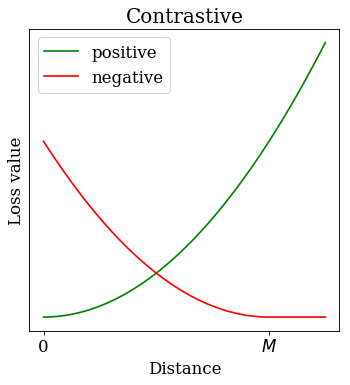
\includegraphics[width=0.48\textwidth]{Figures/contrastive.png}&
        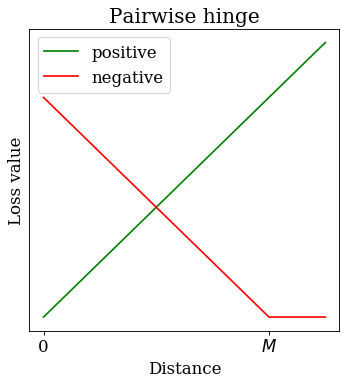
\includegraphics[width=0.48\textwidth]{Figures/pairwise_hinge.png}
    \end{tabular}
    \caption{The values of the Contrastive loss variants: (a) - \eq{contrastive}, (b) - \eq{coherence}. The losses are considered as functions of distance between a pair of image representations. The plots for positive and negative pairs are shown in green and red correspondingly.}
    \label{fig:contrastive}
\end{center}
\end{figure}
Contrastive loss has been first introduced in \citep{hadsell2006dimensionality} for dimensionality reduction and visualization. Later it was used for training a face recognition system in \citep{Sun14} in combination with the cross-entropy classification loss. For a pair of image descriptors $x_i$ and $x_j$ it is defined as:

%todo add more based i=on dimensionality reduction literature (LLE)
\begin{equation}
\label{eq:contrastive}
J_{contrastive}(x_i, x_j) = \begin{cases} \| x_i - x_j \|^{2}_{2}, & \text{if $(i,j)$ is a positive pair,} &\\  (\max(0, M - \| x_i - x_j \|_{2}))^2, & \text{if $(i,j)$ is a negative pair,}\end{cases}
\end{equation}
where $M$ is a hyperparameter, it defines a margin, or minimal distance for a negative pair that does not affect the loss value. In other words, it states when the non-matching examples are far enough and there is no need to push them farther.
The values of the Contrastive loss function for positive and negative pairs are shown in \fig{contrastive}a.

An analogous loss function, called Coherence loss or pairwise hinge loss, was utilized in \citep{mobahi2009deep} and \citep{Simo15} (see \fig{contrastive}b for the corresponding plots):
\begin{equation}
\label{eq:coherence}
J_{coherence}(x_i, x_j) = \begin{cases} \| x_i - x_j \|, & \text{if $(i,j)$ is a positive pair,} &\\  (\max(0, M - \| x_i - x_j \|)), & \text{if $(i,j)$ is a negative pair.}\end{cases}
\end{equation}

However, \citep{Lin15} show that forcing every positive pair to be represented by one point may lead to performance collapse, so the authors introduce the double-margin version of the loss function: 

\begin{equation}
\label{eq:double}
J_{double}(x_i, x_j) = \begin{cases} \max(0,\| x_i - x_j \|^{2}_{2} -M_1), & \text{if $(i,j)$ is a positive pair,} &\\  \max(0, M_2 - \| x_i - x_j \|_{2}^2), & \text{if $(i,j)$ is a negative pair,}\end{cases}
\end{equation}
where $M_1$ and $M_2$ are the two margin hyperparameters for positive and negative pairs correspondingly.\\\\


\bigskip\indent\textbf{Binomial Deviance loss}
 
\begin{figure}
\begin{center}
    \begin{tabular}{cc}
       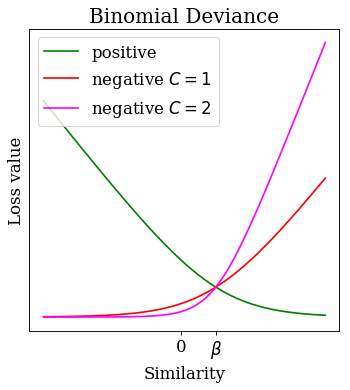
\includegraphics[width=0.48\textwidth]{Figures/bindev.png}&
        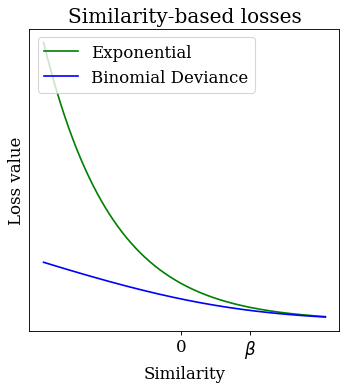
\includegraphics[width=0.48\textwidth]{Figures/similarity.png} \\
        (a) & (b)
    \end{tabular}
    \caption{(a) - the values of the Binomial Deviance loss \eq{bindev}. The plot for negative pairs is shown for $C=1$ and $C=2$, higher values of $C$ mean higher penalty for negative pairs violating the threshold $\beta$. (b) the values of the Binomial Deviance loss \eq{bindev} and the Exponential loss \eq{exp_sim_loss} for positive pairs. The losses are considered as functions of distance between a pair of image representations.}
    \label{fig:bindev}
\end{center}
\end{figure}

Binomial Deviance loss (generalized logistic loss) was considered in \citep{yi2014deep} for training a siamese neural network for person re-identification. Differently to Constrastive loss \eq{contrastive}, it is defined in terms of similarity for a pair of image descriptors. However, it should be noted, that the similar loss was also used in \citep{mignon2012pcca,hu2014discriminative}, but for Euclidean distance instead of cosine similarity. 

Binomial Deviance loss in defined as
\begin{equation}
\label{eq:bindev}
J_{dev}(s_{i,j}) = \ln (\exp^{-\alpha (s_{i,j}-\beta) m_{i,j}} +1 )\,,
\end{equation}
where $s_{i,j}$ is the cosine similarity measure between $i$th and $j$th examples, $\alpha$ and $\beta$ are the hyper-parameters. Furthermore,
$m_{i,j}$ differ for positive and negative pairs: % and scaling factors for the positive and negative pairs, so that:
\begin{align}
    \label{eq:bindev_weights}
    m_{i, j} = \left\{
	\begin{array}{l l}
		1, & \text{if $(i,j)$ is a positive pair,} & \\ 
	   -C, & \text{if $(i,j)$ is a negative pair,} &
	\end{array}\right.
% 	\\
%      w_{i, j}= \left\{
% 	\begin{array}{l l}
% 		\frac {1}{n_1}, & \text{if $(i,j)$ is a positive pair,} &\\
% 		\frac {1}{n_2}, & \text{if $(i,j)$ is a negative pair,} &
% 	\end{array}\right.
\end{align}	
%where $n_1$ and $n_2$ are the number of positive and negative pairs in the training set. 
The parameter $C$ is the negative cost for balancing weights for positive and negative pairs that was introduced in~\citep{yi2014deep}. The authors demonstrate that this parameter may influence the re-identification quality and results in better performance if tuned carefully.
The plots of the Binomial Deviance loss for different similarity values and different values of $C$ are shown in \fig{bindev}a. 

\citep{yi2014deep} have additionally considered the exponential similarity-based loss: 
% \begin{equation*}
%     J_{square}(s_{i,j}) = (s_{i,j} - l)^2,
% \end{equation*}

\begin{equation}
\label{eq:exp_sim_loss}
    J_{exp}(s_{i,j}) = \exp^{-\alpha (s_{i,j}-\beta) m_{i,j}}.
\end{equation}

The corresponding plots for different similarity-based losses are shown in \fig{bindev}b. 
The authors note that $J_{exp}$ \eq{exp_sim_loss} assigns a higher penalty value to the most violating pairs (\ie{} positive pairs with low similarity), whereas $J_{dev}$ \eq{bindev} is more robust to outliers. 

%todo write about classification on same-not same loss 
\citep{Li14, ahmed2015improved} also use binary cross-entropy for pairs of images as an objective. But instead of using a mapping from image to descriptor space first, they map a couple of images straight to the similarity score.

%todo find 2 papers based on comparing distributions


\begin{figure}
\begin{center}
    \begin{tabular}[t]{cc}
    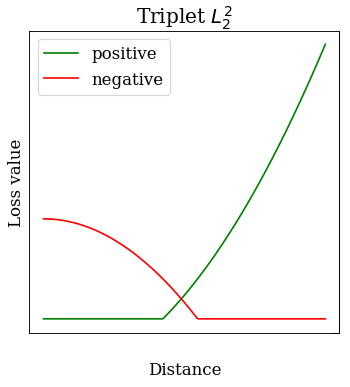
\includegraphics[width=0.48\textwidth]{Figures/triplet_l22.png}&
        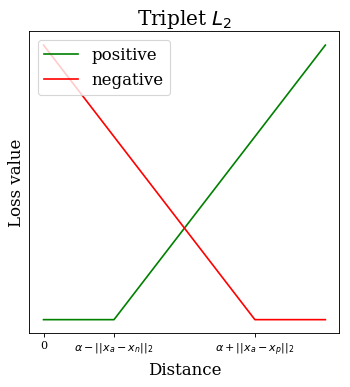
\includegraphics[width=0.48\textwidth]{Figures/triplet_l2.png} 
    \end{tabular}
    \caption{(a) plots the loss \eq{triplet}, (b) plots the loss \eq{triplet_l}. Green and red are for the loss as a function of $\|x_a - x_p \|_2$ and $\|x_a - x_n \|_2$ correspondingly (the other addend remains fixed).}
    \label{fig:triplet}
\end{center}
\end{figure}

\newpage
\bigskip\indent\textbf{Tripletwise losses}\\
\bigskip\indent\textbf{Triplet loss}

\citep{SchroffKP15} and \citep{parkhi2015deep} use the triplet loss (similar to \citep{weinberger2009distance}) for face verification:
\begin{equation}
\label{eq:triplet}
J_{triplet}^{L_2^2}(x_a,x_n,x_p)= \max(0, \alpha - \|x_a - x_n \|^2_{2} + \|x_a - x_p \|^2_{2})
\end{equation}

The loss is defined for a triplet of image representations $x_a$, $x_p$ and $x_n$, where $(x_a,x_p)$ is a positive pairs and $(x_a,x_n)$ is a negative pair. The idea of this loss is different to that of the pairwise losses: now we do not have any predefined threshold (or margin) that should separate all distances between positive pairs from all distances between negative pairs. In the triplet loss, such separation is learned independently for each anchor $x_a$. $\alpha$ is a hyperparameter that forces positive and negative distances to be additionally separated. 

\citep{SchroffKP15} also point out the problem of sampling the training triplets: it is important to select such triplets that violate the condition of the ordering of $x_p$ and $x_n$ in terms of distance to the anchor $x_a$:
\begin{equation*}
    \|x_a - x_p \|^2_{2} + \alpha <  \|x_a - x_n \|^2_{2}
\end{equation*}

In other words, the triplet affects the learning process if the corresponding loss value \eq{triplet} is positive. However, the authors also note that using the hardest (or most violating) triplets may lead to poor performance in practice. Therefore, the semi-hard sampling strategy was suggested. In more details, the triplet $(x_a, x_p, x_n)$ violating a margin $\alpha$ is considered to be semi-hard if the following condition is satisfied:
\begin{equation*}
    \|x_a - x_p \|^2_{2} <  \|x_a - x_n \|^2_{2}
\end{equation*}
Later, it was also shown in \citep{wu2017sampling} that the Contrastive loss \eq{contrastive} also benefits from utilizing this sampling scheme and the final results are on par with those of the triplet loss \eq{triplet}.

\citep{wu2017sampling} argue that the poor results of training using hardest examples come from the concave shape of the loss \eq{triplet} with respect to the distance between the negative pair $D_n = \|x_a - x_n \|_{2}$. The authors point out that the derivative of the loss with respect to $D_n$ is approaching zero for small values of $D_n$, which corresponds to hard triplets. At the same time the derivative of the loss with respect to $D_p = \|x_a - x_p \|_{2}$ remains large. This may lead to imbalance in handling positive and negative components and result in collapsing all representations to one point. \citep{wu2017sampling} suggest that this effect may be reduced by using the following loss function instead:
\begin{equation}
\label{eq:triplet_l}
J_{triplet}^{L_2}(x_a,x_n,x_p)= \max(0, \alpha - \|x_a - x_n \|_{2} + \|x_a - x_p \|_{2})
\end{equation}

The plots for the variants $J_{triplet}^{L_2^2}$ \eq{triplet} and $J_{triplet}^{L_2}$ \eq{triplet_l} are shown in \fig{triplet}.

\bigskip\indent\textbf{Lifted Structured Similarity Softmax loss}

The previously described loss functions are defined for separate pairs or triplets of training examples. The loss values for every such pair or triplet are averaged resulting in the final loss value. Differently from this scheme, \citep{Song16} define the loss function for a whole set of examples. In practice, the loss is calculated for all the examples in the training mini-batch. 

The idea of the \textit{Lifted Structured Similarity Softmax loss} (LSSS) suggested in \citep{Song16} is to take into account the hardest triplets. To make the loss function smooth, the logarithm of the sum of exponents is used. The LSSS loss is defined as follows: 

\begin{equation}
  \begin{aligned}
  \label{eq:lifted}
   J  = \tfrac{1}{2 \left| \mathcal{P} \right|} & \sum_{(i,j) \subseteq \mathcal{P}}  \max(0, \bar{J_{i,j}})^{2}, & \\
    \bar{J_{i,j}}  = \log(& \sum_{(i,k)\subseteq \mathcal{N}} \exp\{\alpha - \|x_i - x_k \|_2\} + &\\
   & \sum_{(j, l)\subseteq  \mathcal{N}}\exp\{\alpha -\|x_j - x_l \|_2\})  + \|x_i - x_j \|_2, & \\
  \end{aligned}
\end{equation}


where $\mathcal{P}$ and $\mathcal{N}$ are the sets of positive and negative pairs in the mini-batch, $\alpha$ is a hyperparameter.

The LSSS loss works with the batch of images and for each positive pair $(x_i, x_j)$ it samples all the related negative pairs $(x_i, x_k)$ and $(x_j, x_l)$. Thus, this approach is based on tripletwise learning. Another feature of this loss is that it is biased towards hard negatives.
%it also does something with mining

\bigskip\indent\textbf{N-pair loss}\\
\citep{sohn2016improved} introduce another loss function based on triplets. 

\begin{equation}
 \label{eq:npair}
 \begin{aligned}
    J_{N-pair}(\{x_i, x_i^+\}_i^N) = \frac1  N \sum_{i=1}^N  \log (1 + \sum_{i \neq j} \exp^{x_i\tran x_j^+ -x_i\tran x_i^+ })\\ = - \frac1  N \sum_{i=1}^N \log \frac {\exp^{x_i\tran x_i^+}}{\exp^{x_i\tran x_i^+} + \sum_{i \neq j} \exp^{x_i\tran x_j^+}}, 
\end{aligned}
\end{equation}
where $\{x_i, x_i^+\}_i^N$ - $N$ example pairs from $N$ different classes.
Similar to LSSS \eq{lifted}, it also uses triplet-based tuple structure where for each example pair multiple negatives are considered.


A similar loss (previously introduced in \citep{goldberger2005neighbourhood,globerson2006metric}), called Proxy-NCA loss, is used by \citep{movshovitz2017no}. The difference is that the positive and negative examples for triplets are replaced by learnable per-class proxies. This results in reduced number of triplets and alleviates the problem of sampling (choosing useful triplets for training). This loss is shown to outperform previously discussed triplet \eq{triplet}, LSSS \eq{lifted} and N-pair \eq{npair} losses.



\bigskip\indent\textbf{Quadruplet losses}
%todo mention that this was suggested simoultaneously or later than our work
%todo_minor: read how the classification problem s harder than verification?

The following loss function is suggested in \citep{Tadmor2016LearningAM} and \citep{wu2017sampling}:

\begin{equation}
\label{eq:margin}
J_{margin}(x_i, x_j) = \begin{cases}  \max(0,\alpha + (\| x_i - x_j \|_{2} - \beta)), & \text{if $(i,j)$ is a positive pair,} &\\  \max(0,\alpha - (\| x_i - x_j \|_{2} - \beta)), & \text{if $(i,j)$ is a negative pair,}\end{cases}
\end{equation}
Where $\alpha$ is a hyperparameter and $\beta$ is a learnable threshold separating the values of distances between positive and negative pairs. This loss is called \textit{margin-based} loss in  \citep{wu2017sampling}, so I follow this notation. Although this loss is defined for a pair of representations $(x_i, x_j)$, it is still related to the quadruplet learning, as the threshold $\beta$ is learned. Note, that the contrastive loss \eq{contrastive} does not allow to learn the margin parameter $M$ as it will converge to zero (the trivial solution). The margin-based loss \eq{margin} also resembles the double-margin contrastive loss \eq{double}.%it also has a trivial soulution if M1 and M2 are not the same!


%+sampling matters and quadruplet loss - the same? yes
%+why M should not be learned in contrastive, but okay for margin-based loss?: hypothesis: in "sampling matters" only  beta_class and beta_i are learned, b_0 remains fixed!- no the reason is that the same beta is used and therefore there is no trivial solution any more
%-+check the multibatch paper-+
%+how the sampling is practically done? - all positives are sampled, for each example in a positive pair, a negative pair is sampled according to the distance weighted sampling procedure.
%todo переделать графики триплето+


%todo say something about sampling
%TODO pcca and bin dev +


%\bigskip\indent\textbf{Other losses}
%center loss
%+ n pairs
%something about local structure?


%one problem is to choose good batches - example magnet loss
%another problem - to sample good examples inside the batch
%there are O(n^3) triplets so there should be more interations to cover all possible triplets, than fow example pairs, but it also has been shown that online sampling and distance reweighting helps triplet training.

%magnet loss uses the same idea of NCA loss, and also use some sort of proxies - clusters. also proxies are used by ProxyNCA and SoftTripleLoss

%softmax loss: it was shown that softmax and 

Besides the loss function choice, another important part of the training scheme is sampling. Hard-negative mining has been initially adopted by \citep{SchroffKP15} for triplet-based learning. Later has been also shown by \citep{wu2017sampling} that the results of contrastive \eq{contrastive} and margin \eq{margin} can be affected by the sampling scheme for negative examples. \citep{wu2017sampling} propose the distance-weighted sampling. \citep{movshovitz2017no}, however, avoid the sampling issue by introducing learnable proxies each of which is representing multiple training data points.



\section{CNN architectures for human recognition}
Several CNN-based methods for person re-identification have been proposed recently: \citep{Li14, yi2014deep, ahmed2015improved, chen2016deep, VariorHW16, VariorSLXW16,SuZX0T16}. 

\citep{yi2014deep} were among the first to build \textit{siamese} architectures that embeds of pedestrian images into the descriptor space, where they can be further compared using angular distance. 

In \citep{yi2014deep}, a peculiar architecture specific to pedestrian images is proposed that includes three independent sub-networks corresponding to three regions (legs, torso, head-and-shoulders). This is done in order to take into account the variability of the statistics of textures, shapes, and articulations between the three regions. %Our architecture includes the network of \citep{yi2014deep} as its part.

Apart from \citep{yi2014deep}, \citep{Li14} and \citep{ahmed2015improved} learn classification networks that can categorize a pair of images as either depicting  the same subjects or different subjects. In both approaches, the two images are fed into the network, and the difference in their mid-level representation is processed by additional special layers. Patch matching layer is used in \citep{Li14} and cross-input neighbourhood difference - in \citep{ahmed2015improved}). After that, extra convolutional and inner product layers are applied to the combined representation of the pair of images. Finally, the classification for the pair of images is performed using the softmax layer. The proposed deep learning approaches \citep{ahmed2015improved, yi2014deep, Li14}, while competitive, do not clearly outperform more traditional approaches based on ``hand-engineered'' features \citep{paisitkriangkrai2015learning, zhao2014person}.

When searching for matches in a dataset, the methods proposed in \citep{Li14}, \citep{ahmed2015improved} and \citep{chen2016deep} need to process pairs that include the query and every image in the dataset, and hence cannot directly utilize fast retrieval methods based on Euclidean and other simple distances. %Here we aim at the approach that can learn per-image descriptors and then compare them with cosine similarity measure. This justifies starting with the architecture proposed in  \citep{yi2014deep} and then modifying it by inserting new layers.
%TODO: VariorHW16, VariorSLXW16,SuZX0T16

Overall, the closest works to our approach described in \chapt{bilinear} are \citep{Yi14,cheng2016person} as they used separate streams to process horizontal stripes of the pedestrian image, both works consider $2$-depth convolutional streams.

The later work \citep{li2017learning} (after our work) use the same approach of multistream CNN (with a deeper $4$-layer architecture), but the authors additionally use Spatial Transformer Networks on each of the substreams, showing the results better than ours. Even better results were shown in \citep{zhao2017spindle}, where a special pose-predicting subnetwork is utilized to propose part-based regions for feature pooling.

\citep{saquib2018pose, suh2018part, kalayeh2018human} continue the idea of using the pose information explicitly. \citep{li2017learning} has a view point predictor as a part of architecture. \citep{suh2018part} and \citep{kalayeh2018human} incorporate sub-networks for pose prediction and semantic segmentation correspondingly.

%in 17 they started to use the pretrained networks!http://openaccess.thecvf.com/content_cvpr_2017/papers/Chen_Beyond_Triplet_Loss_CVPR_2017_paper.pdf http://openaccess.thecvf.com/content_cvpr_2018/papers/Sarfraz_A_Pose-Sensitive_Embedding_CVPR_2018_paper.pdf http://openaccess.thecvf.com/content_cvpr_2018/papers/Kalayeh_Human_Semantic_Parsing_CVPR_2018_paper.pdf http://openaccess.thecvf.com/content_cvpr_2018/papers/Chang_Multi-Level_Factorisation_Net_CVPR_2018_paper.pdf




\section{Multiplicative interactions of features}

\bigskip\ident\textbf{Covariance descriptor and second order pooling}\\
The multiplicative interactions between separate elements of feature vectors have been utilized for different visual recognition tasks. For example, 
the covariance descriptor has been introduced in \citep{tuzel2008pedestrian} for pedestrian detection and was further used for person re-identification and face verification in \citep{ma2012bicov}. 
The covariance descriptor of a region $R$ covering local features $X = \{x_i\}_1^S, x_i \in \mathbb{R}^d$ is defined as:
\begin{equation}
   \label{eq:covariance}
    C_R =\frac{1}{S-1} \sum_{i=1}^{S}(x_i-\mu)(x_i-\mu)\tran
\end{equation}
%compared with first order max and average pooling

Later, in  \citep{carreira2012semantic}, a similar operation has been used to pool the local descriptors in the context of semantic segmentation and classification.  %\citep{tuzel2008pedestrian} and \citep{carreira2012semantic} map the resulting features from the Riemannian manifold of symmetric positive definite matrices to the Euclidean tangent space before learning the final classifiers.

\bigskip\ident\textbf{Bilinear convolutional neural networks}\\
The Bilinear architecture suggested in \citep{lin2015bilinear} are much related to the two aforementioned approaches \citep{tuzel2008pedestrian,carreira2012semantic}). 

%todo fix
The bilinear operation is defined by \eq{bilinear}. It can be noticed that it performs a second-order pooling operation similar to \eq{covariance}.


Differently to \citep{tuzel2008pedestrian} and \citep{carreira2012semantic}, the features outer product is computed for two sets of local features $A$ and $B$ instead of one set of features $X$. The pooling is done over all the spatial locations, so the region $R$ in \eq{covariance} here corresponds to the whole featuremap.  The final architecture can be trained end-to-end which allows to fine-tune the feature extractors.

The Bilinear neural networks are also related to several popular feature aggregation techniques: BoVW \citep{csurka2004visual}, VLAD \citep{jegou2010aggregating} and Fisher Vector \citep{Perronnin10}. The reason is that these methods incorporate the encoding step. Each feature vector is encoded by a number of soft or hard assignments to the corresponding codes in the vocabulary. The resulting descriptor can be represented as an outer product of this encoding and the other part that is specific to the particular aggregation technique. The authors note that such encoding can be also viewed as part detectors. This analogy between the traditional feature aggregation approaches and the Bilinear architecture is described in details in  \citep{roychowdhury2015face}. The authors also show that the Bilinear architecture outperforms the Fisher Vector pooling applied to the local features extracted using a convolutional neural network.

Interestingly, the Bilinear neural networks are able to outperform other methods that rely on the part labeling, \eg{} \citep{branson2014bird}. It should be mentioned that the reported performance is on par with the performance of the Spatial Transformer Network \citep{jaderberg2015spatial}, that may learn the pose normalization without additional pose supervision.

Another important observation made in \citep{roychowdhury2015face} was about the performance of the Bilinear architecture for the birds species categorization. In turned out that the Bilinear architecture performs equally well for the initial images and for their tightly cropped versions. This is a piece of  evidence that the Bilinear model is able to implicitly learn to detect the important image parts.

The authors have initially suggested the Bilinear neural networks for fine-grained recognition problems. These type of recognition is characterized by high intra-category variations and low inter-category variations. The difficulty is that in some cases the intra-category variations may overcome the inter-category ones. For example, when recognizing the bird species, one should be able to take aside the pose and illumination variation an at the same time see the subtle differences in the beak shapes. 

The tasks of human recognition can also be described as fine-grained recognition. Moreover, the Bilinear neural networks have been successfully applied to face recognition with high pose variation in  \citep{lin2015bilinear}. Interestingly, in the latter, it was shown that the Bilinear architecture performs better than simple neural networks even without fine-tuning the feature extractors.  %the feature extractors 

After computing the outer products of the feature vectors, the dimensionality of the resulting feature is squared. This does not constitute a storage or computational problem when operating the low-dimensional features like \citep{tuzel2008pedestrian}, where $8$-length local descriptors were used resulting in the $64$-element covariance matrices. %what about bicov??
But for a large number of feature maps, the result of applying the bilinear operation \eq{bilinear} may be overwhelming. \citep{gao2016compact} address this problem by incorporating Random Maclaurin projection into the deep learning framework, which allows for the lower-dimensional results of the bilinear operation \eq{bilinear} with only a small performance drop.

Later (after the publication of the results of this work), \citep{suh2018part} has  also successfully approached person re-identification using Bilinear architecture. The two feature extractors explicitly model body part detection and appearance recognition: the former has been initialized by the pose detection model of \citep{cao2017realtime}, and the latter - is the GoogLeNet model \citep{szegedy2015going} pre-trained for classification.

%is not cited in introduction because they do not cite us
The latest work in \citep{kalayeh2018human} also applied similar a two-stream-multiplication approach to person re-identification (but is not considered as Bilinear by the authors). Like in the discussed works, one stream extracts appearance information. The other explicitly outputs probability maps for each of the semantic regions associated with different body parts. These maps are used as masks to pool the appearance features inside each semantic region.



\bigskip
\ident\textbf{Attention}\\
Another related line of work aims at explicitly modeling the attention mechanism of perceiving natural sentences and images. At a high level, this can also be described as learning "what" and "where" concepts and combining them using multiplication.

Initially, the simultaneous learning of the deep representations and the corresponding attention weights were introduced in the seminal work of \citep{BahdanauCB14} for neural machine translation. The goal is to encode the input sentence into a sequence of so-called annotation vectors and choose which of them to use (or attend) when generating the next word of the resulting translation. To perform this selection of annotation vectors, a set of corresponding weights is learned. This technique is developed to avoid encoding the whole sentence into a single vector, which leads to poor performance in some cases, \eg{} for long sentences. 

The following work of \citep{xu2015show} use the attention approach to learn visual attention maps for image captioning. \citep{BahdanauCB14} compute annotation vectors for a word sequence as activations of a bidirectional recurrent neural network, similarly, \citep{xu2015show} use a convolutional neural network to produce annotation vectors for a set of image locations.
%todo attention re-id
%todo: the paper citing the ours?

 %face, fine grained recognition

%todo : b-cnn for fine-grained recognition+
%       b-cnn compared to stns & other pose-based models+
%       VLAD FV BoW as bilinear model+-
%       faces with b-cnn: what to mention?-+


%todo other examples of factorization:
%     wavenet?
%gram matrices and style transfer?
%     attention+
%    covariance descriptor+
% todo: deep reid is also here!

\section{Domain adaptation} % and data augmentation

\bigskip\ident\textbf{Domain adaptation}\\
%todo add the notations  from pan2010survey to the introduction???
One popular direction in \textit{transfer learning} is \textit{domain adaptation}. This refers to a case when a  task is being solved for two different domains, as defined in \citep{pan2010survey}. The goal is to adapt the predictive algorithm trained on the labeled source data to the data in the target domain. %todo unsuperwised domain adaptation?

The common assumption in domain adaptation, called \textit{covariate shift} assumption, is that the difference between the two domains mainly comes from the difference in the feature distributions. In more details, under the \textit{covariate shift} assumption, only the marginal distributions of two domains differ, whereas the posterior probabilities of the labels in each domain coincide. This assumption also implies that the feature space is the same for the two domains. Under this assumption, the domain adaptation task is to make the domain marginal distributions closer to each other.   

%\textbf{Maximum Mean Discrepancy}

\citep{huang2007correcting, pan2008transfer, pan2011domain,baktashmotlagh2013unsupervised} estimate the domain distribution difference using Maximum Mean Discrepancy (MMD). The latter has been introduced in \citep{borgwardt2006integrating} to perform the comparison of two samples without the need to estimate the corresponding distributions (in a parametric or non-parametric way). The latter is achieved by utilizing a Reproducing Kernel Hilbert Space (RKHS) and the fact that squared MMD can be expressed in terms of the corresponding kernel function.

The empirical estimate of Maximum Mean Discrepancy is given by:
\begin{equation}
    \label{eq:MMD}
    MMD(X_\S, X_\T) = \| \frac{1}{n_{\S}} \sum_{i=1}^{n_{\S}} \phi \left(x^{\S}_i \right) - \frac{1}{n_{\T}} \sum_{i=1}^{n_{\T}} \phi \left(x^{\T}_i \right) \|_{\mathcal{H}},
\end{equation}
where $\{x^{\S}_i\}_{i=1}^{n_{\S}}$  and $\{x^{\T}_i\}_{i=1}^{n_{\T}}$ are the samples from the source and the target domains correspondingly, $\mathcal{H}$ is RKHS and $\phi$ is the corresponding feature mapping.

However, the mentioned works approach reducing the Maximum Mean Discrepancy differently.
\citep{huang2007correcting} use sample reweighting to choose the most 'useful' examples of the source domain. The idea is to reweight the exampled from the source domain in such a way that the expected risk (associated with the task being solved), for the reweighted source data will be equal to the expected risk for the target data. Such weights are given by $\beta(x,y) = \frac{ P_{\T}(x,y)}{P_{\S}(x,y)}$. And given the covariate shift assumption, $\beta(x) = \frac{ P_{\T}(x)}{P_{\S}(x)}$. To avoid estimating the domain distributions, the authors learn the weights $\beta$ by minimizing the empirical estimate of Maximum Mean Discrepancy between the target domain and the 'reweighted' source domain. 

Differently to \citep{huang2007correcting}, many other approaches seek the transformation of the source feature space (or source and target together) so that the source and target distributions match better. The point of such approaches is to extract the information that
is invariant across the source and target domains. 

\citep{pan2008transfer} aim at finding the lower dimensional space of features for this purpose, the method is called Maximum Mean Discrepancy Embedding. The motivation behind this approach is to get rid of those variation factors of the feature space that cause the marginal distributions of the domains to differ. The authors construct a semidefinite program in terms of the kernel matrix based on \eq{MMD} (with constraints ensuring that the distances between the nearest neighbors are preserved). PCA is then applied to the solution to get the final low-dimensional representations of the source and target examples. One disadvantage of this method is that it does not include any parametrization corresponding to a mapping onto the new feature space, therefore it cannot be used for the out-of-sample data. Such parametrization is introduced in the following work \citep{pan2011domain}, where the learning problem of \citep{huang2007correcting} is reformulated in terms of factorized and parametrized kernel matrix to enable the out-of-sample kernel evaluations. However, this causes the comparison of the sample means in a lower-dimension space rather than in Reproducing Kernel Hilbert Space. A somewhat similar approach correcting this drawback has been suggested in \citep{baktashmotlagh2013unsupervised}. In the latter, the MMD minimization is formulated in terms of the linear projection of the initial data, therefore an explicit transformation of the feature space is learned.

%golapan fernando is also here
While many approaches use Maximum Mean Discrepancy \eq{MMD}, another way of matching different domains is used in \citep{gong2012geodesic}. The authors model the gradual change between the domains. The two domains may have very different axes of variations, therefore the two d-dimensional subspaces, where the corresponding variances for each domain are maximized (\ie{} found using PCA), will be far from each other on the Grassmann manifold. The goal is to explore the intermediate subspaces on this manifold to extract the domain-invariant features. Moreover, the authors apply the kernel trick to take into account all the intermediate subspaces along the curve connecting the source and target domains. %is there any explicit mapping to a new feature space? yes it is shown in gong2013connecting (just square root of the kernel matrix)

The resampling technique similar to \citep{huang2007correcting} is utilized in \citep{gong2013connecting} in combination with the approach of \citep{gong2012geodesic}. The approach is based on the idea of solving multiple easier domain adaptation subtasks and then using their solutions as a basis for the final domain-invariant representation. Subtasks correspond different combinations of the examples in each of the two domains: to formulate each subtask, some examples are removed from the source domain and added to the target domain. Such examples are denoted \textit{landmarks} and are chosen by thresholding the results of sample reweighting (each subtask - with different kernel parameters). Therefore the examples from the source domain that are closest to the target domain are chosen in different ways. This allows to solve easier adaptation tasks, moreover, this gives multiple different perspectives on the initial task. The representations achieved by solving each of the subtasks are scaled and concatenated, and the scaling weights are learned discriminatively using the landmark examples and their labels.


\bigskip\ident\textbf{Deep domain adaptation}
%problem the re-id in the context of da is nor modelled

\bigskip\ident\textbf{Feature-level domain adaptation.} Like many of the above-mentioned methods, deep learning methods for domain adaptation aim at learning a data representation that would be the best at explaining both domains simultaneously. However, deep learning gives the tools for learning such features at multiple levels, whereas non-deep techniques work with data descriptions that are fixed and extracted beforehand. Deep learning methods, in contrast, are able to work with the raw input and extract a hierarchy of features. Thus, like for many other recognition tasks, multiple successful deep learning methods have been suggested for domain adaptation. 

One of the first deep domain adaptation methods was suggested in \citep{glorot2011domain} for sentiment analysis. The Denoising Autoencoder \citep{vincent2008extracting} is trained on the mixed data from both domains to capture their common concepts. Like in the non-deep approaches, described above, the transformed labeled data are then used for training the final domain-invariant classifier.

\citep{chopra2013dlid} combines the ideas of \citep{gong2012geodesic} and \citep{glorot2011domain} to propose a deep learning framework interpolating between the two domains. Unlike \citep{glorot2011domain}, both the task-specific prediction algorithm and domain-invariant feature extractors are neural networks. This allows finetuning the parameters of both these parts simultaneously by propagating the gradients from the task-specific network to the feature extractors. The gradual change between the domains is modeled by constructing multiple variants of the mixture of the two domains: different proportions of the data from the two domains are used. Each of the feature extractors is trained in an unsupervised manner using one of such mixtures. The final representation is composed as a concatenation of outputs of all of these feature extractors.

Finally, \citep{LongC0J15} suggest a deep neural network, called DAN (Deep Adaptation
Network), that is trained with the two objectives: one is a task-specific loss and another is to match the distributions of the two domains using Maximum Mean Discrepancy \eq{MMD}. The matching is performed for several higher-level layers of the main neural network to ensure that the domains are aligned well, as the last layers of a neural network are considered to be the most domain-specific ones. \citep{tzeng2014deep} similarly use \eq{MMD} as an additional objective to train a domain-invariant neural network. In the latter, the authors use only one layer for matching the domain distributions. This layer is chosen among the last layers of the neural network so that the corresponding MMD value is minimized.

Notably, the deep approaches of \citep{chopra2013dlid, tzeng2014deep, LongC0J15} outperform the previous non-deep methods, \eg{} the strong method of \citep{gong2012geodesic}, by a large margin on the cross-domain classification.
%todo which of them are better? compared to non-deep?

\bigskip\ident\textbf{Image-level domain adaptation.}
%to do last layers are
%this is extracted from da face paper
%todo: rewrite ?
%model
Since the CycleGAN \citep{ZhuPIE17} architecture for image-to-image translation and stylization appeared, domain adaptation has become one of its active fields of application. This approach differs from the feature-level domain adaptation techniques of \citep{LongC0J15} and \citep{tzeng2014deep} or the method presented in the \chapt{gradrev}, because rather than finding deep domain-invariant representations, it works on the pixel level and aims at building mappings between the image domains. Thus the domain adaptation is done in two steps: building a mapping the source domain to target and retraining the predictor on the transferred source data. (Although it is also possible to combine these two steps into one optimization process.)%cycada


The methods of \citep{Hoffman17,Deng_2018_CVPR,Murez_2018_CVPR} employ CycleGAN framework to change the domain of training data for various tasks, including classification, segmentation, and person re-identification. 

%pedestrians
In particular, for person re-identification, the pixel-level domain adaptation with CycleGAN has been applied in several recent works \citep{zhong2018camera, Deng_2018_CVPR} (after the results of the \chapt{gradrev} were published). Some of them consider different datasets as domains, others aim at utilizing synthetic re-identification data to improve the results on real data \citep{bak2018domain}. As demonstrated by these works, image-to-image translation may help a lot to overcome the visual (\eg{} caused by different illumination) differences between the source and target camera sets.


 \citep{HongIRY17} and
 \citep{SohnLZY0C17} approach face recognition tasks for low-quality image domain. They consider image degradation as a domain shift and perform feature-level unsupervised domain adaptation based on adversarial learning showing better recognition results. 
In works \citep{HongIRY17} and \citep{SohnLZY0C17} it is shown that domain-specific data augmentation is essential for training face recognition systems. 
 However, in both works, the data augmentation is performed 'by hand' (the degradation types and hyper-parameters for transforms are chosen and fixed).%, while we augment the training data in an automatic manner utilizing the CycleGAN framework, which can also be viewed as an image-level domain adaptation.
%Additionally, in contrast to \citep{HongIRY17}, we do not consider extremely large pose variation. Instead, we are more focused on the image degradation factors (e.g. the combination of small size, blur, JPEG-compression). 
%Differently from \citep{SohnLZY0C17}, where evaluation is performed for the Youtube faces dataset, we approach the task in the presence of the somewhat stronger domain shift, as our test data are captured by surveillance cameras and are mostly of much lower quality.


%\subsection{Adversarial learning for augmentation}

%todo in hist loss check the @cumber@ problem if there are too many bins (and some are empty)